\chapter{Research Methodology}\label{ch:methodology}

\section{Research design}\label{sec:design}

The project follows an experimental, comparative design. Rather than proposing
a new algorithm, it measures how well existing NLP and LLM techniques perform
on one concrete task: identifying and typing semantic relationships between
the provisions of \standardA{} and \standardB{}. All methods are run on the
same extracted dataset and scored against the same ground truth, so
differences in the results can be attributed to the methods themselves.

The design addresses the research questions directly. RQ1 (feasibility and
limits of automated relationship identification) is answered by the absolute
performance levels and the error analysis. RQ2 (comparison of method families)
is answered by evaluating all eleven methods under identical conditions. RQ3
(automated vs.\ expert mapping) is answered by treating the reference annotation
as the standard of comparison and additionally measuring how consistently the
task is performed on repetition. The expert role in that comparison is filled by
LLM-assisted annotation reviewed by the authors against a written codebook, not
by external domain experts; a protocol for the external study is given in
Appendix~\ref{app:survey} but was not carried out, and Section~\ref{sec:threats}
states what this costs the RQ3 answer.

The workflow has five stages --- extraction, ground-truth construction,
automated mapping, evaluation, and reporting --- described in the remainder of
this chapter and implemented in the pipeline of Chapter~\ref{ch:prototype}.

\section{Data: standards and provision extraction}\label{sec:data}

\subsection{Source documents}

Both standards are publicly available from ETSI. \standardA{} v3.1.3 defines
baseline security provisions for consumer IoT devices; \standardB{} v2.1.1
defines baseline security requirements for AI models and systems. The two
documents differ in structure and terminology but share a numbered-provision
format, which the extraction step exploits.

\subsection{Extraction of normative provisions}

Security standards mix normative requirements with explanatory prose,
examples, and notes. Only the normative statements are relevant for mapping,
so the first step isolates them. The PDF documents are converted to plain text
with \texttt{pdftotext}, recurring page headers and footers are stripped, and
provisions are located by their clause identifiers (e.g., ``Provision
5.3-3'' in \standardA{}, numbered requirement clauses in \standardB{}). For
each provision the pipeline records: the provision identifier, source
standard, section number and title, the full provision text, and its modality
--- whether the provision uses \emph{shall} (mandatory), \emph{should}
(recommended), or \emph{may} (permitted).

The extraction yields 69 provisions from \standardA{} and 72 from \standardB{},
141 in total. Since any provision of one standard could in principle relate to
any provision of the other, the mapping space contains $69 \times 72 = 4{,}968$
candidate pairs. Extraction correctness was checked by sampling provisions and
comparing them against the original PDFs; counts per section were also
compared with the tables of contents of both standards.

Text preprocessing is deliberately minimal. The transformer models used in
this project expect natural sentences and apply their own tokenisation, so
provisions are passed to them essentially as extracted. Only the TF--IDF
baseline applies lowercasing and English stop-word removal as part of its
vectoriser. Domain terms (authentication, encryption, integrity,
vulnerability, and so on) are never stripped, since they carry the meaning the
mapping depends on.

\section{Relationship taxonomy}\label{sec:taxonomy}

Every candidate pair $(a, b)$, with $a$ from \standardA{} and $b$ from
\standardB{}, is assigned exactly one of six relationship types:

\begin{description}[style=nextline]
  \item[\textsc{Equivalence}] $a$ and $b$ express the same security objective
  with comparable scope.
  \item[\textsc{Subsumption (A broader)}] $a$ covers the objective of $b$ and
  more; $b$ is a special case of $a$.
  \item[\textsc{Subsumption (B broader)}] the converse: $b$ covers $a$.
  \item[\textsc{Overlap}] the provisions share part of their objective, but
  each also covers ground the other does not.
  \item[\textsc{Complementarity}] the provisions address different aspects
  that jointly support a common security goal, without overlapping scope.
  \item[\textsc{No relation}] no meaningful connection.
\end{description}

Full definitions with decision guidance appear in
Appendix~\ref{app:labels}. For evaluation, the two directional subsumption
labels are merged into a single \textsc{Subsumption} class, since direction
confusions are less interesting than detecting subsumption at all and the per
-direction supports are small.

\section{Ground-truth construction and validation}\label{sec:gt}

\subsection{LLM-assisted annotation}

Evaluating the automated methods requires a reference mapping. Annotating all
4{,}968 pairs manually was outside the scope of a 15-credit project, so the
ground truth was produced with LLM assistance and human review, a set-up
increasingly common in annotation work and disclosed here for transparency.
Candidate pairs and draft relationship labels were generated with Claude Opus~5
(Anthropic), prompted with the full provision texts and the taxonomy
definitions of Section~\ref{sec:taxonomy}. The authors then reviewed the
drafts, corrected labels and justifications, and removed pairs whose
connection did not hold up against the original standard texts. Each retained
pair carries a short written justification and a reviewer confidence score
from 1 (uncertain) to 3 (certain).

The resulting ground truth contains 107 pairs: 85 positive pairs (3
equivalence, 51 overlap, 9 subsumption across both directions, 22
complementarity) and 22 explicit \textsc{No relation} pairs. The negative
pairs were chosen to be non-trivial --- provisions that share surface
vocabulary but differ in objective --- so that methods relying on word overlap
are actually tested. The class distribution is skewed towards
\textsc{Overlap}, which reflects the real relationship between a device-level
and a life-cycle-level standard: near-identical requirements are rare.

Using an LLM in the annotation loop creates a risk of circularity, since one
of the evaluated methods is itself an LLM. Two design choices reduce this
risk: the annotation model (Claude) is from a different family than the
evaluated model (Gemini), and the labels follow a codebook written before any
were drafted. Human review, however, covers only the 107 pilot pairs. The
650-pair probability sample of Section~\ref{sec:sampling} was not reviewed pair
by pair --- at that size it would have consumed the project's remaining budget
--- so its reliability rests on the blind comparison against the reviewed pilot
reported in Section~\ref{sec:gtvalidation}. The residual risk is examined there
and discussed in Section~\ref{sec:threats}.

\subsection{A probability sample of the candidate space}\label{sec:sampling}

The pilot set of Section~\ref{sec:gt} was assembled purposively, by examining
pairs that looked promising. That makes it useful for developing the method and
unusable for estimating anything about the corpus: its pairs have no inclusion
probabilities, so its 79.4\% positive rate cannot be corrected toward the rate a
deployed system would meet. A second reference set was therefore drawn as a
probability sample.

Pairs were first ordered by a screening score: the mean percentile rank of each
pair across all five similarity matrices. Averaging over the methods keeps the
strata neutral between them. Stratifying on one model's scores would instead
sample densely wherever that model is confident, and quietly flatter it at
evaluation. The ordered space was then cut into three strata and sampled at
deliberately unequal rates.

\begin{table}[htbp]
\centering
\caption{Stratified sampling design over the 4{,}968 candidate pairs. Unequal
allocation concentrates annotation where relations are common while keeping every
inclusion probability strictly positive, which is what keeps the estimator
unbiased.}
\label{tab:sampling}
\small
\begin{tabular}{lrrrr}
\toprule
Stratum & Screening rank & $N$ & $n$ & Weight $N/n$\\
\midrule
H & top 10\%    &   497 & 250 & 1.99\\
M & next 30\%   & 1\,490 & 200 & 7.45\\
L & bottom 60\% & 2\,981 & 200 & 14.91\\
\midrule
  &             & 4\,968 & 650 & \\
\bottomrule
\end{tabular}
\end{table}

Each pair stores its stratum and weight, so corpus-level precision, recall,
specificity and prevalence follow by Horvitz--Thompson estimation, with
confidence intervals from a bootstrap that resamples within stratum. Batches are
shuffled under a fixed seed before annotation, so a partially completed pass is
still a random subsample rather than a biased prefix. All 650 designed pairs were
annotated, in 19 batches of 40, together with the 107 pilot pairs mixed into the
same stream.

Disproportionate allocation buys efficiency at a price in variance. The weights
span 1.99 to 14.91, giving a Kish design effect of 1.49: the 650 pairs carry the
information of about 437 drawn with equal probability. This is reported alongside
the estimates in Section~\ref{sec:prevalence} rather than left implicit, since a
weighted sample whose nominal size is quoted without its design effect overstates
its own precision.

Annotation followed a written codebook fixed before labelling began, reproduced
in Appendix~\ref{app:labels}. It states the decision procedure, the
overlap-versus-complementarity test that carries most of the difficulty, and one
amendment made partway through and applied from that point onward. The 107 pilot
pairs were mixed into the stream unmarked, so re-labelling them was blind and
their agreement with the earlier author-reviewed labels can be read as a check on
the new annotation (Section~\ref{sec:agreementresults}).

\begin{figure}[htbp]
\centering
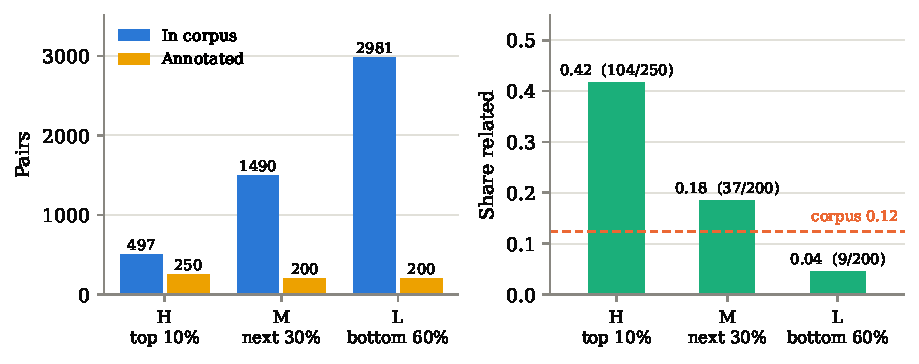
\includegraphics[width=\textwidth]{figures/stratum_yield}
\caption[Sampling strata and observed yield]{Left: size of each stratum in the
candidate space against the number of pairs annotated from it. Right: the share
of annotated pairs in each stratum carrying a relationship, with the
weighted corpus estimate for reference. The monotone gradient across strata is
evidence that the screening score orders the space as intended; the corpus
estimate sits below all but the lowest stratum because that stratum holds three
pairs in five.}
\label{fig:strata}
\end{figure}

Figure~\ref{fig:strata} shows the realised sample. The stratum yields (0.42,
0.18, 0.04) confirm the screening score separates the space, and they are also
why the design is efficient: an unstratified sample of the same size would spend
three annotations in five on a region where one pair in twenty-five is related.

One class stayed out of reach. The sample contains no \textsc{Equivalence} pair
at all, despite covering half of the top-decile stratum, so no weighted per-class
estimate can be given for it; the three instances in the corpus known to the
project all come from the purposive pilot. That is itself a measurement --- two
standards written for different layers of a system produce overlapping and
complementary obligations, but almost never identical ones --- and it is the
reason per-class results in Section~\ref{sec:classresults} are reported on the
pilot set only.

\subsection{Reliability of the reference set}\label{sec:gtvalidation}

Three statistics are reported, all computable from what was actually done. The
first is agreement between the sample and the author-reviewed pilot labels on the
pairs they share, using raw agreement and Cohen's kappa~\cite{cohen1960kappa}
with the bands of Landis and Koch~\cite{landis1977kappa}. The second is
calibration: whether recorded annotation confidence predicts where the two label
sets diverge. The third is a contrast rather than a validation --- the
run-to-run self-agreement of the evaluated LLM on identical input, which
establishes what an unreliable annotation source looks like on the same scale.

Cross-model agreement using Gemini is deliberately excluded. Gemini is one of the
evaluated methods, so its labels cannot serve as an independent check on a
reference set used to score it.

A larger validation with external cybersecurity professionals was designed but
not executed within the project timeframe; the complete survey instrument and
analysis plan are provided in Appendix~\ref{app:survey} as a ready-to-run
protocol for future work.

\section{Automated mapping methods}\label{sec:methods}

Eleven methods are evaluated, grouped into five families. The grouping is not
housekeeping: it is what the comparison is about. Lexical baselines match
words. Sentence-embedding models are trained so that cosine similarity means
something. Contextual-embedding models are masked language models pooled into a
vector without any such training. A cross-encoder reads both provisions at once
and answers a directional question. Hosted API models are the commercial
current generation. Differences within a family isolate the effect of the
model; differences between families isolate the effect of the approach.

\subsection{Rule-based baselines}

\paragraph{TF--IDF cosine similarity.} Each provision is represented as a
TF--IDF-weighted bag of words; every cross-standard pair receives the cosine
similarity of the two vectors. This captures shared vocabulary and nothing
else, making it the canonical lexical baseline.

\paragraph{Security-keyword Jaccard.} A curated list of cybersecurity terms
(password, authentication, encryption, vulnerability, logging, risk, update,
and others) is matched against each provision; a pair is scored by the Jaccard
overlap of the keyword sets. This baseline mimics how a checklist-driven
analyst might shortlist related provisions.

\subsection{Sentence-embedding models}

Three encoders trained so that cosine similarity between sentence embeddings
tracks semantic relatedness. Each provision is embedded once and every pair is
scored by the cosine of the two vectors.

\begin{itemize}
  \item \textbf{Sentence-BERT} (\texttt{all-MiniLM-L6-v2})
  ~\cite{reimers2019sbert}, the compact model that made this style of
  comparison cheap enough to run over a full pair space;
  \item \textbf{MPNet} (\texttt{all-mpnet-base-v2})~\cite{song2020mpnet}, the
  strongest general-purpose model of the same family, included so that the
  effect of model capacity can be separated from the effect of the task;
  \item \textbf{BGE} (\texttt{bge-base-en-v1.5})~\cite{xiao2024bge}, a
  retrieval-trained embedder a generation newer than the other two, included as
  the current state of the open embedding literature.
\end{itemize}

\subsection{Contextual-embedding models}

Three masked language models with no sentence-similarity training, mean-pooled
over token embeddings and L2-normalised. They are included to separate two
explanations for embedding performance that are easily confused --- the size of
the model, and whether it was ever trained to make its geometry mean something.

\begin{itemize}
  \item \textbf{BERT} (\texttt{bert-base-uncased})~\cite{devlin2019bert}, the
  general-purpose baseline;
  \item \textbf{SecureBERT}~\cite{aghaei2022securebert}, a
  cybersecurity-domain RoBERTa model;
  \item \textbf{CySecBERT}~\cite{bayer2024cysecbert}, a second, independently
  built cybersecurity-domain model. One domain-adapted model that behaves oddly
  is an anecdote about that model; two, adapted by different groups from
  different base models, make it a statement about domain adaptation for this
  task.
\end{itemize}

\subsection{Cross-encoder inference}\label{sec:nlimethod}

Every method above reduces a pair to one symmetric number, and a symmetric
number cannot say which of two provisions is the broader one. Subsumption is
therefore unreachable for all of them by construction. The
\textbf{NLI cross-encoder} (\texttt{nli-deberta-v3-base}, a DeBERTa-v3
model~\cite{he2023debertav3} fine-tuned on natural language inference
data~\cite{williams2018mnli}) reads both provisions together and returns
whether the first entails the second, which is a directional question.

Each pair is scored twice, once in each direction, and the two entailment
probabilities decide the label: entailment both ways is
\textsc{Equivalence}; entailment one way only is \textsc{Subsumption} with the
entailed provision as the narrower one; some entailment but not enough in
either direction is \textsc{Overlap}; and no entailment either way is
\textsc{No relation}. A direction counts as entailed at probability $0.50$, and
$0.20$ is the floor below which the method emits nothing at all. Both cut-offs
were fixed before any evaluation. The stored score is the larger of the two
entailment probabilities, so this method can be swept and recalibrated on the
same footing as the others. The cost is two forward passes per pair, 9{,}936 in
total, against one embedding pass per provision for the bi-encoders.

\subsection{Hosted API methods}

\paragraph{Gemini embeddings.} Each provision is embedded with Google's
\texttt{gemini-embedding-2} model via API; pairs are scored by cosine
similarity, exactly as for the local encoders. This represents the current
generation of commercial embedding models.

\paragraph{Gemini LLM classification.} For every one of the 4{,}968 pairs, a
prompt containing both provision texts and the six label definitions asks
\texttt{gemini-2.5-flash-lite} to answer with exactly one label. Jobs are
submitted through the batch API. Unlike the similarity methods, this approach
predicts a relationship type directly and can, in principle, distinguish
overlap from complementarity --- something a scalar similarity cannot.

\subsection{From similarity scores to labels}\label{sec:thresholds}

The similarity-based methods produce scores in $[0,1]$, not labels. Scores are
mapped to relationship types with fixed thresholds: $\geq 0.85$
\textsc{Equivalence}, $\geq 0.70$ \textsc{Overlap}, $\geq 0.50$
\textsc{Complementarity}, otherwise \textsc{No relation}. A second, lower
threshold decides whether a pair is emitted as a candidate at all, and it is
set per family rather than per model: $0.10$ and $0.05$ for the two lexical
baselines, $0.30$ for the sentence-embedding models, $0.70$ for the
contextual-embedding models, $0.50$ for the Gemini embeddings, and the
entailment floor of Section~\ref{sec:nlimethod} for the cross-encoder. These
cut-offs follow the operating points reported in related mapping work
~\cite{sapkota2016regcmantic}, and they are fixed per family rather than tuned
per model so that a difference between two models in the same family reflects
the representation and not the calibration.

That decision has a consequence worth stating in advance rather than
discovering in the results. A threshold chosen a priori is a threshold chosen
without knowing the base rate of related pairs, and
Section~\ref{sec:prevalence} shows the base rate is far lower than the pilot
set suggests. Several methods therefore ship at operating points that are badly
wrong for the corpus, which is why every method with a continuous score is also
reported at a threshold recalibrated on the probability sample. The threshold
sensitivity analysis in Section~\ref{sec:thresholdresults} shows how much of
each method's performance is representation and how much is calibration.

Subsumption cannot be expressed as a symmetric similarity band at all, so ten
of the eleven methods cannot predict it by construction. Only the cross-encoder
can, which is the reason it is in the study.

\section{Evaluation framework}\label{sec:evaluation}

Evaluation is restricted to the 107 annotated pairs; predictions outside the
annotated set are ignored, since their true labels are unknown. Two views are
computed for every method.

\subsection{Pair detection}

Detection asks whether a method finds related pairs at all, regardless of
label. A pair is a positive if its ground-truth label is anything but
\textsc{No relation}. With $TP$, $FP$, $FN$ counted within the annotated
scope:
\begin{equation}
  \text{Precision} = \frac{TP}{TP+FP}, \qquad
  \text{Recall} = \frac{TP}{TP+FN}, \qquad
  F_1 = \frac{2PR}{P+R}.
\end{equation}
One consequence of scoping deserves emphasis: false positives can only be
counted on the 22 annotated negative pairs. A method that predicts relations
sparsely can therefore show precision of 1.0 while missing nearly everything;
precision values must be read together with recall and with the
predicted-positive counts reported alongside.

\subsection{Relationship classification}

Classification asks whether the predicted label matches the ground truth,
over all 107 pairs, with the subsumption directions merged
(Section~\ref{sec:taxonomy}). Ground-truth pairs absent from a method's
output count as predicted \textsc{No relation}. Reported metrics are overall
accuracy and macro-averaged precision, recall, and F1 over the five classes,
plus per-class scores. Macro averaging weights all classes equally, which is
appropriate here because the rare classes (equivalence, subsumption) are
exactly the ones a compliance analyst cares most about.

\subsection{Uncertainty and sensitivity}

With 107 evaluation pairs, point estimates alone would overstate certainty.
Nonparametric bootstrap confidence intervals (2{,}000 resamples of the
annotated pairs, percentile method, 95\% level) are reported for detection F1
and macro-F1. For every method with a stored similarity matrix, detection
metrics are additionally computed across the full threshold range
$[0.05, 0.975]$ to separate the quality of the underlying representation from
the choice of operating point.

Corpus-level results are reported at two operating points, because the shipped
thresholds were selected on the pilot set and applying them to a corpus with a
different base rate confounds the method with its calibration. The second point
is chosen on the probability sample itself: weighted F1 is maximised on four
folds and scored on the fifth, over 20 repeats, with folds stratified by
sampling stratum so each carries all three weight classes. Candidate cut-offs
are quantiles of each method's own score distribution rather than a shared
absolute grid, since the methods occupy ranges that differ by an order of
magnitude in width. The reported threshold is the median of the 100 selections,
so the point estimate that follows is not the in-sample optimum; the gap between
it and the cross-validated mean is reported as the residual optimism.

Comparisons between methods use a paired bootstrap on the difference: both
methods are scored on the same within-stratum resample, and only differences
whose interval excludes zero are reported as orderings. Two marginal intervals
overlapping is not evidence that the methods are equivalent, because the
methods are scored on identical pairs and their errors are correlated.

Which comparisons are made is decided by a rule, not by inspection. Eleven
methods and their recalibrated variants admit more than two hundred pairwise
contrasts, and two hundred uncorrected 95\% intervals will contain false
findings whatever the data say. Two questions carry the argument --- whether a
method beats the all-positive baseline, and whether anything beats the
best-scoring method --- so each method is compared against those two references
and against nothing else. One caveat attaches to the second reference: it is
selected as the maximum on this sample, and a difference measured against a
selected maximum is biased in that maximum's favour, because the selection
absorbs part of the sampling noise. Those intervals describe the gap to the
leader; they are not a test that the leader is genuinely best.

\subsection{Efficiency and interpretability}

Wall-clock runtime of each stage is recorded on commodity hardware (Apple
silicon laptop, CPU only). Interpretability is assessed qualitatively: whether
a method's output carries any human-readable rationale (matched keywords, a
similarity score, or a generated label) that an analyst could act on.
